\subsection{Algorithm outline}

\subsubsection{Analysis}

The analysis algorithm is as follows:

\begin{enumerate}
	\item Get configuration, initialize global variables.
	\item Check the following:
	\begin{enumerate}
		\item Do the user settings make sense? If not, exit.
		\item Are the paths to the input file and the programs correct? If not, exit.
		\item Do the output directories exist? If not, create them.
		\item Does the database structure exist? If not, exit.
	\end{enumerate}
	\item Backup old results, if requested.
	\item Clear old results from file system and database, if requested.
	\item Create the HMMs, if they do not exist.
	\item Create the BLAST database of all core taxa, if it does not exist.
	\item Configure the hmmsearch and BLAST modules.
	\item Translate the input file in all six reading frames, if it is nucleic acid data.
	\item Load the translated sequences into the database, generating unique SHA256
		digests on the way.
	\item Get all translated sequences of the target species from the database.
		Sequence identifiers are now SHA256 digests. Write the sequences into a
		Fasta file.
	\item For each HMM, do the following:
	\begin{enumerate}
		\item Search the translated sequences with this HMM. Read the tabular search
			report and store it in the database. Skip to the next HMM if no hits were
			obtained.
		\item For each hit, do the following:
		\begin{enumerate}
			\item Get the hit sequence from the database and write the relevant
				subsequence to a Fasta file. This information has been gained from the
				hmmsearch report file.
			\item Search this sequence against the BLAST database. Read the tabular
			search report and store it in the database. Skip to the next HMM if no
			hits were obtained.
		\end{enumerate}
	\end{enumerate}
	\item Print some statistics and exit.
\end{enumerate}

\subsubsection{Reporting}

The reporting algorithm is as follows:

\begin{enumerate}
	\item Get configuration, initialize global variables.
	\item Get a list of ortholog group IDs and their associated ortholog sequences
		from the database.
	\item Get all results in the form:
	\begin{lstlisting}
	hmmsearch_evalue => {
		ortholog_group_id => [
			reciprocal_hit,
			reciprocal_hit,
		],
		ortholog_gene_id => [
			reciprocal_hit,
			reciprocal_hit,
		],
	}
	\end{lstlisting}
	\item Sort the e-values in ascending order.
	\item Starting with the lowest hmmsearch e-value, do the following:
	\begin{enumerate}
		\item For each ortholog group that has a hit with this e-value, do the following:
		\begin{enumerate}
			\item Check whether this ortholog group is present in the list that was
				generated in step 2. If not, skip to the next group (this ortholog group
				has already been assigned a transcript).
			\item Sort the reciprocal hits by BLAST e-value in ascending order.
			\item For each reciprocal hit, do the following:
			\begin{enumerate}
				\item If the reciprocal search hit a sequence that is in this ortholog
					group, and this transcript has not been assigned previously, then this
					is a valid match. Otherwise, skip to the next reciprocal hit unless
					the ``soft threshold'' has been reached (in that case, skip to the
					next ortholog group).
				\item Assign this transcript to this ortholog group. Neither can be
					assigned again.
			\end{enumerate}
		\end{enumerate}
	\end{enumerate}
\end{enumerate}

\subsection{Database design}

\subsubsection{Advantages of using a relational database}

\pname uses a MySQL relational database management system (RDBMS) for fast and
efficient sequence data storage and retrieval. The introduction of a RDBMS has a
number of advantages over file-based sequence storage:

\begin{description}
	\item[Memory efficiency.] The sequence data does not need to be loaded into
		RAM for fast access since the DBMS manages sequence storage and retrieval.
		This becomes especially important when analyzing data files larger than the
		computer's physical memory.
	\item[No redundancy.] Every sequence and each orthology relationship is stored
		in the database exactly once with a unique identifier. 
	\item[Speed.] The DBMS is highly optimized for speed and efficiency. If
		configured correctly, complex joins comprising millions of rows are
		executed quickly due to the use of B-tree indices.  %TODO MySQL performance
	\item[Flexibility.] SQL queries allow custom-tailored filtering and output.
\end{description}

The database was structured in a way that reduces redundant information to a
minimum. A structure diagram is shown in Figure \ref{fig:dbstructure}.

\begin{figure}[ht]
	\begin{center}
		%\includegraphics[width=\textwidth]{img/db-structure.pdf}
	\end{center}
	\caption{Database structure.}
	\label{fig:dbstructure}
\end{figure}

\subsection{Algorithmic decisions}

\subsubsection{Checksums guarantee uniqueness}

As outlined on page \pageref{uniq}, unique sequence IDs are necessary in
order for \code{hmmsearch} not to create confusion by treating whitespace in
sequence headers as a description separator. To avoid this, and to maintain a
consistent naming scheme across applications, \pname~uses a SHA-256 checksum to
generate a unique ID for every sequence. The checksum is generated using both
the original header and the sequence. Sequences are loaded into the database
along with these checksums. During the analysis, wherever a file is generated
that includes sequence identifiers, this checksum is used. This also eliminates
the problem with \code{fastatranslate} introducing whitespace that might confuse
\code{hmmsearch}.

It must be guaranteed that no two checksums, i.e., two sequence identifiers, are
ever the same. The SHA-256 hashing algorithm generates a checksum that is 160 bits,
or 40 hexadecimal characters in length. The probability $p$ of a hash collision
(i.e., two hashed elements returning the same checksum) in $n$ elements is

\begin{equation}
p \ge \frac{n (n-1)}{2} \times \frac{1}{2^b}
\label{eq:hashcollision}
\end{equation}

where $b$ is the number of bits generated by the hash function. There need to be
more than $1.7 \times 10^{15}$ objects for the SHA-256 hashes to exceed a collision
probability of $10^{-18}$. Since the hash space is expected to contain only a
number of objects in the range of $10^6$ to $10^{12}$, it is statistically safe
to assume that every checksum is unique. 

\subsubsection{Traversing the hit list by e-value}

The candidate orthologs are sorted by the e-value of their respective HMM
search. By doing so, it is assured that the most relevant candidate is assigned
a transcript. This avoids a ``first come, first serve'' scenario in which a
candidate with a high e-value gets assigned a transcript that is then no longer
available for a candidate with a lower e-value.

\subsubsection{Removing hits from the candidate list eliminates redundancy}

In order to avoid redundant assignment, i.e., a single transcript being assigned
to multiple ortholog groups or vice versa, candidate pairs that have been
verified are removed from the list of candidates. 

\begin{figure}[ht]
	\begin{center}
		%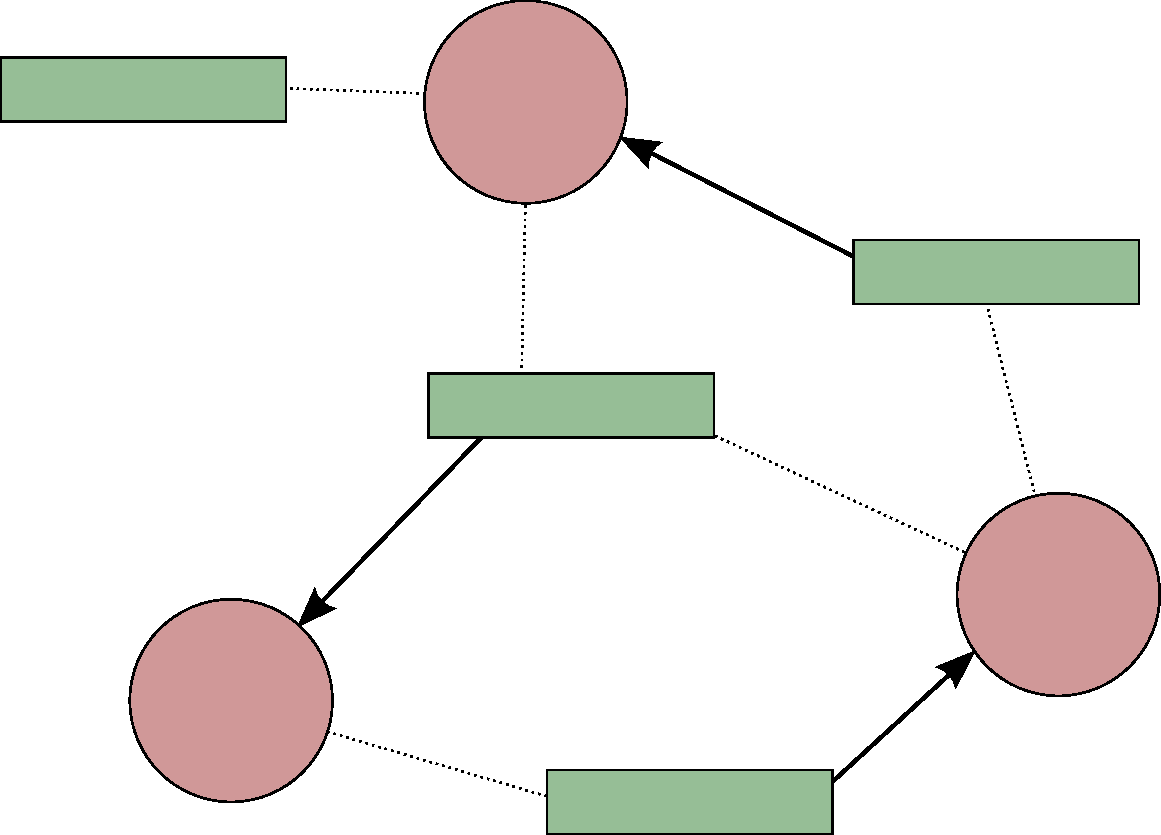
\includegraphics[width=0.8\textwidth]{img/orthograph_graph.pdf}
	\end{center}
	\caption{A two-dimensional graph. The ortholog groups (OG) are connected to the
	candidate hit transcripts by the e-value of the HMM search. Traversing the graph
	by e-value and assigning the transcripts to the OG with the best
	hit results in transcript 2 being assigned to OG A, transcript 3 to OG B and
	transcript 4 to OG C. Transcript 1 remains unassigned because the HMM search
	e-value for OG A is higher than the e-value for transcript 2.}
	\label{fig:graph}
\end{figure}
